\section{Supporting infrastructure}

\noindent In order to support more frequent software releases, a number of supporting tools and techniques need to be put in place. A sub-set of such tools and techniques are already deployed by technical coordinator to support the testbed 1 of the project. The technical coordinator is responsible for establishing and managing the toolset.\\

\noindent The saman Github repo plays a vital role in the production of software releases. In order to support more frequent software releases the repo must continue to be active between the scheduled testbed integration phases. Its activity in any interim periods will not be so intense, but rapid response to integration issues will be important.\\

\noindent The technical coordinator has already put in place a number of tools and techniques to ease software integration and the production of the software release for testbed 1. These include a code repository, communication platform (Slack) and an incident tracking processing (Github issue management). Further steps can be taken to reduce integration effort by catching potential conflicts earlier in the development cycle. Such measures, as with the software itself, will be extended with each release and subject to more detailed planning.\\

\noindent As a means of providing feedback on integration issues to software developers in each release as early as possible, the aim is to put in place mechanisms to automatically build, test and document all the software on a daily basis. Such “nightly builds” are for the benefit of the team developers and hence will not be systematically distributed to the application groups and users since they will not be the subject of the release testing procedure (see below). However, the contents and status of the nightly builds will be available to everyone in the project via tools such as Travis-CI.

\subsection{Centralised code repository}

\noindent Many of the tools and techniques foreseen within the software infrastructure are linked to the use of a code repository. In the build-up to testbed 1, team members have to produce commits containing their software to either the saman central repository or their own repositories that are then mirrored into the \texttt{dev} branch before merging to \texttt{master} branch.\\

\noindent This central repository will act as the core facility on which the automated building, testing and documentation tools will be based. It is essential that all team members adopt the code repository as an integral part of their daily working practises. Sustained software development without committing modifications to the central repository for extended periods (weeks) will undermine the functioning and value of the nightly build procedure.\\

\noindent To enable the use of several of the proposed tools and to simplify browsing, the source code should be stored in the repository as individual files. The application can then be produced as one of the final parts of the build procedure.\\

\noindent It is expected that detailed documentation including code descriptions, class hierarchies and dependencies can be extracted from comments in the source code and by auto-documentation tools. More high-level documentation will still need to be written by hand. All documentation, both extracted and hand-written, will evolve with each software release. To ensure users get the correct version of the hand-written documentation for a software release it will be necessary to archive the documentation, preferably in the same repository as the code itself. This implies using documentation formats (e.g., separate \LaTeX\: or Dart Docstrings / documentation and style documentation files, e.g. .css, .html or .js) that lends themselves to archiving tools such as Github.  

\subsection{Development branch}

A development branch is required in order to support iterative development, integration and testing without interfering with the validation activities performed by the stakeholders in the \texttt{master} branch. In the current planning, it is foreseen that commits for development or integration work will first be committed to the \texttt{dev} branch before any merges are done to the \texttt{master} branch. The daily development versions of any branches in the software can be tested at any time by any of the team members. It is recommended that all team members get to know the development done on each active branch in the saman central repository. The overall progress and status of the development branch will be managed by technical coordinator in conjunction with the team members.\\

\noindent If a developer wants to add features to the saman project he needs to branch from the \texttt{dev} branch and name the branch in accordance with the following naming convention \texttt{feature\_name\_1}. Ones the feature is ready for deployment to \texttt{dev} it can be merged. It needs to be emphasized that any merges to the \texttt{dev} branch must be done through a \texttt{pull\_request\_1} (PR) where all developers except the creator of the PR are assigned roles as reviewers. Ones all \texttt{pull\_requests} are merged to the \texttt{dev} branch and the team feels confident in the content of the \texttt{dev} branch and the release date has come then the application is ready to be released (\texttt{release\_1}), i.e. merge \texttt{dev} with the \texttt{master} branch. The illustration below (Figure \ref{fig:git_flow}) shows the relation between \texttt{feature}, \texttt{dev} and \texttt{master} branches.\\

\noindent All branches must remain available to the developers for the duration of the project. If a branch is to be deleted this must be confirmed and agreed upon by the technical coordinator.

\begin{figure}
\centering


\tikzset{every picture/.style={line width=0.75pt}} %set default line width to 0.75pt        

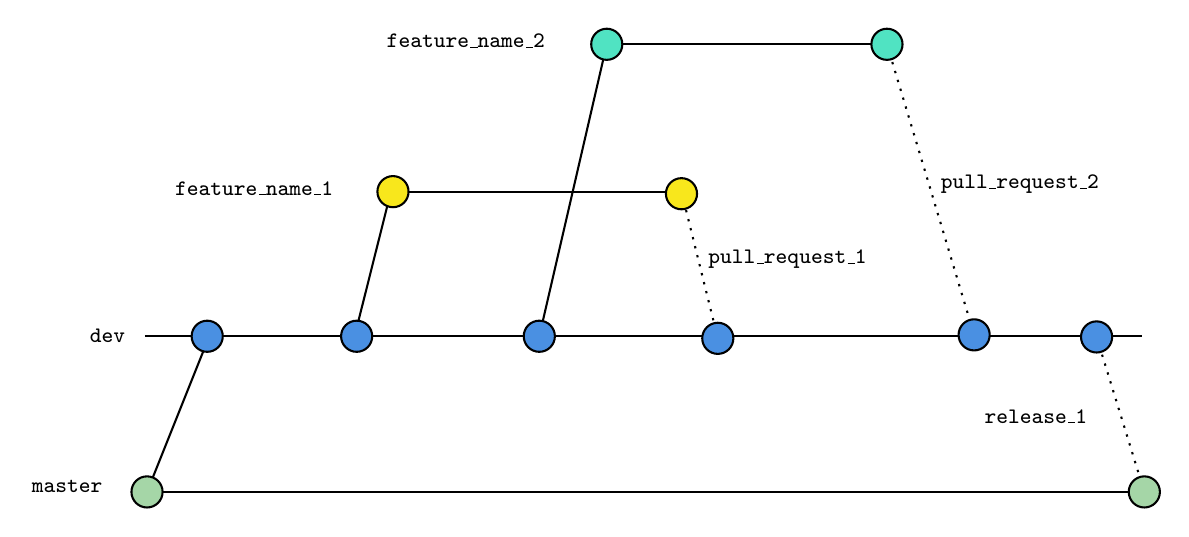
\begin{tikzpicture}[x=0.75pt,y=0.75pt,yscale=-1,xscale=1]
%uncomment if require: \path (0,440); %set diagram left start at 0, and has height of 440

%Straight Lines [id:da41312231801086075] 
\draw    (100,306) -- (581.5,306) ;
%Straight Lines [id:da2699367760381708] 
\draw    (100,231) -- (580.5,231) ;
%Straight Lines [id:da46769746764105635] 
\draw    (101,306) -- (131,231) ;
%Shape: Circle [id:dp2689759381912853] 
\draw  [fill={rgb, 255:red, 74; green, 144; blue, 226 }  ,fill opacity=1 ] (122.5,231) .. controls (122.5,226.86) and (125.86,223.5) .. (130,223.5) .. controls (134.14,223.5) and (137.5,226.86) .. (137.5,231) .. controls (137.5,235.14) and (134.14,238.5) .. (130,238.5) .. controls (125.86,238.5) and (122.5,235.14) .. (122.5,231) -- cycle ;
%Shape: Circle [id:dp9796387627490961] 
\draw  [fill={rgb, 255:red, 165; green, 214; blue, 167 }  ,fill opacity=1 ] (93.5,306) .. controls (93.5,301.86) and (96.86,298.5) .. (101,298.5) .. controls (105.14,298.5) and (108.5,301.86) .. (108.5,306) .. controls (108.5,310.14) and (105.14,313.5) .. (101,313.5) .. controls (96.86,313.5) and (93.5,310.14) .. (93.5,306) -- cycle ;
%Straight Lines [id:da3524961791886829] 
\draw    (218.5,161.33) -- (358.5,161.33) ;
%Straight Lines [id:da6953964199151648] 
\draw    (218.5,161.33) -- (201,231) ;
%Shape: Circle [id:dp19505024316180086] 
\draw  [fill={rgb, 255:red, 248; green, 231; blue, 28 }  ,fill opacity=1 ] (212,161.33) .. controls (212,157.19) and (215.36,153.83) .. (219.5,153.83) .. controls (223.64,153.83) and (227,157.19) .. (227,161.33) .. controls (227,165.48) and (223.64,168.83) .. (219.5,168.83) .. controls (215.36,168.83) and (212,165.48) .. (212,161.33) -- cycle ;
%Shape: Circle [id:dp8567875642277254] 
\draw  [fill={rgb, 255:red, 74; green, 144; blue, 226 }  ,fill opacity=1 ] (194.5,231) .. controls (194.5,226.86) and (197.86,223.5) .. (202,223.5) .. controls (206.14,223.5) and (209.5,226.86) .. (209.5,231) .. controls (209.5,235.14) and (206.14,238.5) .. (202,238.5) .. controls (197.86,238.5) and (194.5,235.14) .. (194.5,231) -- cycle ;
%Straight Lines [id:da4444663602056733] 
\draw  [dash pattern={on 0.84pt off 2.51pt}]  (376,232) -- (358.5,161.33) ;
%Shape: Circle [id:dp8314560296395388] 
\draw  [fill={rgb, 255:red, 74; green, 144; blue, 226 }  ,fill opacity=1 ] (368.5,232) .. controls (368.5,227.86) and (371.86,224.5) .. (376,224.5) .. controls (380.14,224.5) and (383.5,227.86) .. (383.5,232) .. controls (383.5,236.14) and (380.14,239.5) .. (376,239.5) .. controls (371.86,239.5) and (368.5,236.14) .. (368.5,232) -- cycle ;
%Shape: Circle [id:dp5049389788192327] 
\draw  [fill={rgb, 255:red, 248; green, 231; blue, 28 }  ,fill opacity=1 ] (351,162.33) .. controls (351,158.19) and (354.36,154.83) .. (358.5,154.83) .. controls (362.64,154.83) and (366,158.19) .. (366,162.33) .. controls (366,166.48) and (362.64,169.83) .. (358.5,169.83) .. controls (354.36,169.83) and (351,166.48) .. (351,162.33) -- cycle ;
%Straight Lines [id:da06393516926407528] 
\draw    (322.5,90.33) -- (290,231) ;
%Shape: Circle [id:dp7073671514314899] 
\draw  [fill={rgb, 255:red, 74; green, 144; blue, 226 }  ,fill opacity=1 ] (282.5,231) .. controls (282.5,226.86) and (285.86,223.5) .. (290,223.5) .. controls (294.14,223.5) and (297.5,226.86) .. (297.5,231) .. controls (297.5,235.14) and (294.14,238.5) .. (290,238.5) .. controls (285.86,238.5) and (282.5,235.14) .. (282.5,231) -- cycle ;
%Straight Lines [id:da36314281016924843] 
\draw    (322.5,90.33) -- (457.5,90.33) ;
%Shape: Circle [id:dp8333157814110803] 
\draw  [fill={rgb, 255:red, 80; green, 227; blue, 194 }  ,fill opacity=1 ] (315,90.33) .. controls (315,86.19) and (318.36,82.83) .. (322.5,82.83) .. controls (326.64,82.83) and (330,86.19) .. (330,90.33) .. controls (330,94.48) and (326.64,97.83) .. (322.5,97.83) .. controls (318.36,97.83) and (315,94.48) .. (315,90.33) -- cycle ;
%Straight Lines [id:da9736022589266866] 
\draw  [dash pattern={on 0.84pt off 2.51pt}]  (457.5,90.33) -- (499.5,230.33) ;
%Shape: Circle [id:dp692663884634666] 
\draw  [fill={rgb, 255:red, 80; green, 227; blue, 194 }  ,fill opacity=1 ] (450,90.33) .. controls (450,86.19) and (453.36,82.83) .. (457.5,82.83) .. controls (461.64,82.83) and (465,86.19) .. (465,90.33) .. controls (465,94.48) and (461.64,97.83) .. (457.5,97.83) .. controls (453.36,97.83) and (450,94.48) .. (450,90.33) -- cycle ;
%Shape: Circle [id:dp542003916280043] 
\draw  [fill={rgb, 255:red, 74; green, 144; blue, 226 }  ,fill opacity=1 ] (492,230.33) .. controls (492,226.19) and (495.36,222.83) .. (499.5,222.83) .. controls (503.64,222.83) and (507,226.19) .. (507,230.33) .. controls (507,234.48) and (503.64,237.83) .. (499.5,237.83) .. controls (495.36,237.83) and (492,234.48) .. (492,230.33) -- cycle ;
%Straight Lines [id:da5568825658870458] 
\draw  [dash pattern={on 0.84pt off 2.51pt}]  (558.5,231.33) -- (581.5,306) ;
%Shape: Circle [id:dp7539785128233116] 
\draw  [fill={rgb, 255:red, 74; green, 144; blue, 226 }  ,fill opacity=1 ] (551,231.33) .. controls (551,227.19) and (554.36,223.83) .. (558.5,223.83) .. controls (562.64,223.83) and (566,227.19) .. (566,231.33) .. controls (566,235.48) and (562.64,238.83) .. (558.5,238.83) .. controls (554.36,238.83) and (551,235.48) .. (551,231.33) -- cycle ;
%Shape: Circle [id:dp178100284508252] 
\draw  [fill={rgb, 255:red, 165; green, 214; blue, 167 }  ,fill opacity=1 ] (574,306) .. controls (574,301.86) and (577.36,298.5) .. (581.5,298.5) .. controls (585.64,298.5) and (589,301.86) .. (589,306) .. controls (589,310.14) and (585.64,313.5) .. (581.5,313.5) .. controls (577.36,313.5) and (574,310.14) .. (574,306) -- cycle ;

% Text Node
\draw (113,155) node [anchor=north west][inner sep=0.75pt]  [font=\footnotesize] [align=left] {{\footnotesize \texttt{feature\_name\_1}}};
% Text Node
\draw (72,226) node [anchor=north west][inner sep=0.75pt]  [font=\footnotesize] [align=left] {{\footnotesize \texttt{dev}}};
% Text Node
\draw (44,299) node [anchor=north west][inner sep=0.75pt]  [font=\footnotesize] [align=left] {{\footnotesize \texttt{master}}};
% Text Node
\draw (370,188) node [anchor=north west][inner sep=0.75pt]  [font=\footnotesize] [align=left] {{\footnotesize \texttt{pull\_request\_1}}};
% Text Node
\draw (215,84) node [anchor=north west][inner sep=0.75pt]  [font=\footnotesize] [align=left] {{\footnotesize \texttt{feature\_name\_2}}};
% Text Node
\draw (482,152) node [anchor=north west][inner sep=0.75pt]  [font=\footnotesize] [align=left] {{\footnotesize \texttt{pull\_request\_2}}};
% Text Node
\draw (503,265) node [anchor=north west][inner sep=0.75pt]  [font=\footnotesize] [align=left] {{\footnotesize \texttt{release\_1}}};


\end{tikzpicture}

\caption{Github workflow}
\label{fig:git_flow}
\end{figure}

\subsection{Toolset}

Recommendations including guidelines/templates and examples for the use of tools and techniques to support automated building, testing and documentation are currently in preparation. Such a toolset will provide a convenient, standardised, project-wide mechanism for building the software and documentation. It is important that all the team members adopt the toolset as early as possible. The details of this toolset are defined in below, but this list is a non-exhaustive list of these tools and techniques:

\begin{itemize}
\item Mark-up techniques (e.g., Dart style comments) for document generation from source code;
\item A tool capable of extracting formatted source comments and producing documentation in various formats (e.g., Android Studio build in linters);
\item A web interface for browsing the repository (e.g., Google Chrome);
\item Github issue management for problem reporting and tracking;
\item Test harnesses (e.g., codecov etc.);
\item Build tools (e.g., Travic CI etc.) capable of constructing the software on all supported platforms and producing RPMs for distribution;
\item A “slack repo notifier” providing a daily digest of commits to the repository from all team members;
\item A web page providing access to the results of the most recent automated build, test and documentation cycle;
\item Coding style recommendations and tools for checking them (e.g., Dart lint);
\end{itemize}

\noindent The tools at the top of the list are the highest priority and work using them is already started by the team members.\\

\noindent All tools or techniques will be set-up by the technical coordinator using the centralised code repository as a basis and will be deployed in a step-wise manner. It is not intended to develop new tools to support the nightly builds but rather configure existing widely used tools. In this manner, development by team members can be concentrated on exploiting such tools and techniques in their daily work without worrying about the installation and support issues for the tools they use.
